\section{KeyGraph Algorithm}
Extracting keywords from a document is not an easy task with normal tools[9], we use Keygraph Algorithm to solve the problem. In Keygraph, we extract keywords representing the asserted main point in a document, without relying on external devices such as natural language processing tools or a document corpus. It is based on Graph Segmentation, representing co-occurrence relationships among terms in the document, forming clusters. Each cluster corresponds to the concepts that the author's ideas are based on, and the top terms are chosen as keywords based on the statistics of each word's relation to these clusters. Because it only uses the idea of graph and statistic, it works very fast to extract keywords.\\
To build a building, we need a foundation. And the walls, the doors and windows, and all kinds of decorations. However, the nature of the building is to protect the inhabitants from solar radiation and Rainstorm on the roof. To support the roof, we need some more columns.\\
Similarly, to write a good document, we first need to know that the basic concept of the document is based on the first step. The detailed description needed to configure documents, metaphors, and samples is also essential. Last but not least, in order to emphasize the main points, such as the column of a building, it is also necessary to deploy content in the document.\\
Keygraph uses the idea of building, and have the features as follow[5]:
\begin{enumerate}
\item expressing the main point of the author, not frequent terms.
\item using only information in the text of documents without NLP tools.
\item working very fast.
\end{enumerate}
There are three steps to achieve the algorithm.
\begin{enumerate}
\item extracting foundations: basic and preparatory concepts are obtained as clusters base on the co-occurrence nouns.
\item extracting columns: the relationships between nouns and concepts are obtained.
\item extracting roofs and keywords: nodes at the cross of strong columns.
\end{enumerate}
When we have a document, we call it $D$, is composed of sentences, which are in turn composed of words.\\
Beforehand, we have a noise list of non-significant words, which have less meaning. We call it stop words list and it contains words such as `a', `and', `here', etc. We also need to transform words to original form, for example, `do', `doing', and `does', are same words, we need to reduce them all to `do'. Then our $D$ is represented by $D_{terms}$ include unique terms, $D_{terms} = \{w_1, w_2, w_3,...\}$, each term is a word or a phrase in $D_{terms}$. Then we can start our algorithm.[5]\\ \\
\textbf{Extracting\ Foundations}\\ \\
We need to make a Graph $G$ for document $D$, which is made of nodes representing terms, and the links representing the co-occurrence. First, the nodes are high-frequency terms in $D$, and they become the candidates of the foundation. We choose the top-30 high-frequency terms as nodes and, we call them $HF$. That means terms in $HF$ become terms in $G$. We link the nodes in $HF$ if their association is strong, here, we define the association of terms $w_i$, and $w_j$ in $D$, as
\begin{displaymath}
assoc(w_i,w_j) = \sum_{s \in \mathcal{D}} min(|w_i|_s, |w_j|_s),
\end{displaymath}
where $|x|_s$ means the count of $x$ in sentence $s$. After that, we have built our foundations. It doesn't matter whether $G$ is a connected graph or not. We call the connected ones, clusters.
\begin{figure}[!hbp]
\centering
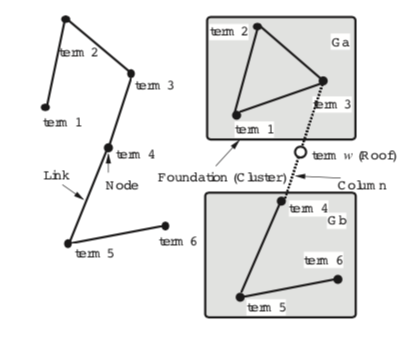
\includegraphics[width=250pt]{./pictures/0203.png}
\caption{Extracted foundations as $G_a$ and $G_b$}
\end{figure}
\\ \\
\textbf{Extracting\ Columns}\\ \\
Keywords that we want are important terms that can hold all the clusters. We assign value $key(w)$ for each term $w$ in document $D$. $key(w)$ in a number between 0 and 1, which is defined as the probability of term $w$ to appear if all the foundations in $G$ are considered. We have defined $|x|_s$ as the count of term $x$ in sentence $s$, we also have $|g|_s$, which is the count of cluster $g$ in sentence $s$, as the count of terms in $s\cap g$. We define based and neighbors as,
\begin{displaymath}
based(w,g) = \sum_{s \in \mathcal{D}}|w|_s|g-w|_s
\end{displaymath}
\begin{displaymath}
neighbors(g) = \sum_{s\in \mathcal{D}}\sum_{w\in s}|w|_s|g-w|_s
\end{displaymath}
where,
\begin{displaymath}
|g-w|_s = |g|_s - |w|_s,\ if \ w \in g
\end{displaymath}
$based(w,g)$ is the co-occurrence degree between term $w$ and other terms in cluster $g$. $neighbor(g)$ is the count of terms in sentences including terms in $g$.\\
base on these functions, $key(w)$ is defined as follow,
\begin{displaymath}
key(w)=1-\prod_{g\in \mathcal{G}}(1-base(w,g)/neighbors(g))
\end{displaymath}
That means,
\begin{displaymath}
key(w) = probability(w|\bigcap_{g \subset \mathcal{G}}g)
\end{displaymath}
or it is logically equivalent to that,
\begin{displaymath}
key(w) = probability(\bigcup_{g\subset \mathcal{G}}(w|g))
\end{displaymath}
Sorting all the terms in $D$ by keys produces a list of terms ranked by their association with the clusters. We choose top-12 key terms as high key terms.\\ \\
\textbf{Extracting\ Roofs,\ Keyword}\\ \\
After works before, we need to add all the high key terms as new nodes to $G$, of course, if they are not in $G$ yet. The keywords are not high keys, there may exist especially important foundations are of low keys but highly ranked by the sum of the strength of touching columns. We still have some other processing. Column is a value between a high key term $w_i$ and a high-frequency term $w_j$, as
\begin{displaymath}
column(w_i,w_j)=\sum_{s\in \mathcal{D}}min(|w_i|_s,|w_j|_s)
\end{displaymath}
We can sort them by $column(w_i,w_j)$ for columns touching $w_i$, for each high key term $w_i$. columns with highest column values and connecting term from two different clusters are selected to create new links. and finally, we make a keygraph for a document.\\
Nodes in $G$ are sorted by the sum of columns. We choose top-12 terms as the keywords that extracted by KeyGraph Algorithm.
We have realized the algorithm by Python language, in the section after, we will have some experiment on evaluating the result of KeyGraph, Here we have a simple example of KeyGraph on Japanese stories.
\begin{figure}[!hbp]
\centering
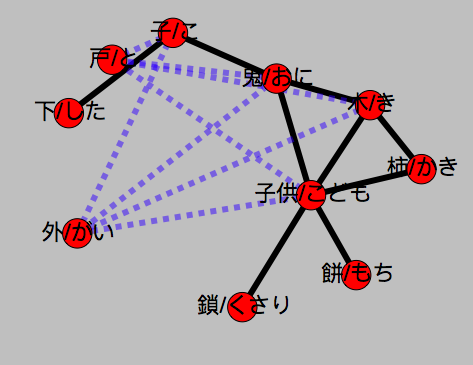
\includegraphics[width=250pt]{./pictures/0203-1.png}
\caption{an example of KeyGraph}
\end{figure}